The details of the numerical setup are presented in Section \ref{f1}.

Each element has $m_V=9$ vertices so in total $ndof_V\times m_V=18$ velocity dofs and 
$ndof_P*m_P=4$ pressure dofs. The total number of 
velocity dofs is therefore $NfemV=nnp \times ndofV$ while the total number of
pressure dofs is $NfemP=nel$. The total number of dofs is then $Nfem=NfemV+NfemP$.

As a consequence, matrix $\K$ has size $NfemV,NfemV$ and matrix $\G$ has size $NfemV,NfemP$.
Vector $f$ is of size $NfemV$ and vector $h$ is of size $NfemP$.  

\begin{center}
\includegraphics[width=12cm]{python_codes/fieldstone_18/q2q1setup}\\
{\color{red} renumber all nodes to start at zero!! Also internal numbering does not work here }
\end{center}

\fbox{
\parbox{10cm}{{\bf features}
\begin{itemize}
\item $Q_2\times Q_1$ element \index{$Q_2 \times Q_1$}
\item incompressible flow \index{incompressible flow}
\item mixed formulation \index{mixed formulation}
\item Dirichlet boundary conditions (no-slip)
\item isothermal \index{isothermal}
\item isoviscous \index{isoviscous}
\item analytical solution \index{analytical solution}
\end{itemize}
}}

\begin{center}
\includegraphics[width=10cm]{python_codes/fieldstone_18/errors}
\end{center}
